\documentclass[12 pt]{book}
\usepackage{amsmath}
\usepackage{amsthm}
\usepackage[paperwidth=5 in,paperheight=5 in,left=6 mm, right=6 mm, top=15 mm, bottom=22 mm]{geometry}
\usepackage{graphics}
\usepackage{fontawesome}
\usepackage{enumitem}
\usepackage{marvosym}
\newcommand{\myitem}{\refstepcounter{enumi}\item[$^\star$\theenumi.]}
\newcommand{\mmyitem}{\refstepcounter{enumi}\item[$^{\star \star}$\theenumi.]}
\setcounter{page}{01}

\usepackage[utf8]{inputenc}
\usepackage{xcolor}
\setlength{\arrayrulewidth}{0.1 mm}
%BLUE%
%\definecolor{Mycolor2}{HTML}{3D9BE9}
\definecolor{Mycolor2}{HTML}{33cccc}
%\definecolor{Mycolor2}{HTML}{000000}

%%----HEADER &&& FOOTER----%%

\usepackage{fancyhdr}


\pagestyle{fancy}
\fancyhf{}
\setlength{\headheight}{8 mm}
%\fancyhead[CE,CO]{ \Times\Large{\textbf{\textls*[100]{\textcolor{tomato}{\textit{Illustration}}}}}}

\fancyhead[CE,CO]{\Large{\textbf{\textls*[250]{\textcolor{tomato}{SOLVE ME! \\[-5 mm]{\Large{\textbf{\textls*[5000]{\textcolor{black}{\scalebox{.42}{ROTATION}}}}}}     }}}}}


\fancyfoot[CE,CO]{\Large{\textls*[10]{\textcolor{tomato}{\Times\textit{\tikz \draw [-{Stealth[red]}, line width=4.5,line cap=round] (0,0) node[below=-13.5 mm,scale=2.2,below left]{\textbf{Solution}}--(1.65,0);}}}}}

\renewcommand{\headrulewidth}{0 mm}
\renewcommand{\footrulewidth}{0 mm}


\DeclareMathOperator{\Ln}{ln}

%%----FONT &&& MATHS_FONT----%%

\usepackage{amssymb}
\usepackage{upgreek,xspace}
\newcommand*{\rom}[1]{\expandafter\@\romannumeral #1}


\usepackage[utopia]{mathdesign}
\renewcommand{\familydefault}{\sfdefault}
\usepackage[scaled=1]{helvet}
\newcommand*\Times{\fontfamily{ptm}\selectfont}

%%%------PACAKAGES------%%%

\usepackage[letterspace=120]{microtype}
\usepackage{enumitem}
\usepackage{multicol}
\usepackage{pgfplots}
\pgfplotsset{width=8cm,compat=1.16}
\usepackage{tikz}
\usepgfplotslibrary{fillbetween}
\usetikzlibrary{quotes,angles,patterns,through,calc}
\usepgflibrary{arrows.meta}
\usetikzlibrary{decorations.pathmorphing}
\usetikzlibrary{decorations.markings}
\usetikzlibrary{arrows.meta,bending}
\usepackage{rotating}
\usepackage{tikz-3dplot}
\include{tikz-3dplot}
\usepackage[american voltages, american currents,siunitx]{circuitikz}
\usepackage{circuitikz}
\usetikzlibrary{fit,positioning}
\usetikzlibrary{optics}
\usetikzlibrary{intersections}
\usetikzlibrary{decorations.pathreplacing}
\usepackage{setspace}
\setstretch{1.1}
\usepackage{tkz-tab} [3]



\usepackage{vwcol}[widths={0.25,0.75}]


\usepackage{color}
\usepackage[autostyle]{csquotes}


\usepackage{xcolor}
\definecolor{Mycolor2}{HTML}{33cccc}
\definecolor{One}{HTML}{336666}
\definecolor{Two}{HTML}{666666}
\definecolor{Three}{HTML}{cc6699}


%  black--brown--black %
\definecolor{Four}{HTML}{000000}
\definecolor{Five}{HTML}{330000}
\definecolor{Six}{HTML}{000000}

\definecolor{Seven}{HTML}{ff6666}
\definecolor{Eight}{HTML}{330066}
\definecolor{Nine}{HTML}{cc3333}
\definecolor{tomato}{HTML}{FF6347}
\definecolor{darkblue}{HTML}{2c3e50}
\definecolor{blackm}{HTML}{363636}
\definecolor{pink}{HTML}{ff6666}






  \tikzset{every to/.style={append after command={[draw,dashed]}}}

\tikzset{
  mirror->/.style={postaction={decorate,black!95,draw,thick,
decoration={border,amplitude=-0.25cm,angle=45,segment length=0.22cm}}
  }
}



\def\centerarc[#1]#2(#3)#4(#5:#6:#7)% [draw options] (center) (initial angle:final angle:radius)
  {\draw[#1]($(#3)+({#7*cos(#5)},{#7*sin(#5)})$)arc(#5:#6:#7);}



\newcommand{\sm}{\begin{minipage}[c]{0.1\linewidth}
{\Huge{\textcolor{tomato}{\textbf{ }}}}
\end{minipage}}

\newcommand{\AxisRotator}[1][rotate=0]{%
    \tikz [x=0.25cm,y=0.60cm,line width=.2ex,-stealth,#1] \draw (0,0) arc (-120:120:1 and 1);%
}


%%%%%%       Problem Number        %%%%%%%%
%%%%%%       Problem Number        %%%%%%%%

\newcommand{\nm}{\begin{minipage}[c]{0.1\linewidth}
{\Huge{\textcolor{tomato}{\textbf{20. }}}}
\end{minipage}}

%%%%%%       Problem Number        %%%%%%%%
%%%%%%       Problem Number        %%%%%%%%

\newcommand{\vl}{{{\textcolor{tomato}{\textbf{\vrule width 2.25 pt{}}}}}}

\newenvironment{question}
{	
	\nm  \vl \,
	\begin{minipage}[l]{0.86\linewidth}
	\begin{itshape}
	\large\Times\textit{}
}
{
	\end{itshape}
	\end{minipage}
}


\newenvironment{options}
{	
	\sm ~
	\begin{minipage}[l]{0.86\linewidth}
	\begin{multicols}{2}
	\begin{enumerate}[label={(\roman*)}, itemsep=4 mm]
	\normalsize{}
}
{
	\end{enumerate}
	\end{multicols}
	\end{minipage}
}


\newenvironment{v-options}
{	
	\sm ~
	\begin{minipage}[l]{0.86\linewidth}
	\begin{enumerate}[label={(\roman*)}, itemsep=4 mm]
	\normalsize{}
}
{
	\end{enumerate}
	\end{minipage}
}



\newenvironment{definition}
{
	\begin{center}
	\begin{itshape}
	\normalsize\Times\textit{}
}
{
	\end{itshape}
	\end{center}
}


\newenvironment{note}
{
	\begin{center}
	\begin{itshape}
	\normalsize\Times\textit{}
}
{
	\end{itshape}
	\end{center}
}


\newenvironment{calculations}
{
	\begin{itshape}
	\normalsize\Times\textit{}
}
{
	\end{itshape}
}


\newenvironment{q-options}
{	
	\sm ~
	\begin{minipage}[l]{0.86\linewidth}
	\begin{note}
	\begin{enumerate}[label={(\roman*)}, itemsep=1 mm]
	\normalsize{}
}
{
	\end{enumerate}
	\end{note}
	\end{minipage}
}



\newcommand{\physics}{\normalsize{\textcolor{tomato}{\textls*[100]{{\hspace*{75 mm} @10xphysics}}}}}
\newcommand{\solution}{\centering\Large\Times\textbf{\textcolor{tomato}{\textls*[100]{ \textit{\\[-20 mm]Solution}}} }}
\newcommand{\calculation}{\centering\large\Times{\textcolor{tomato}{ \textit{\\[-18 mm]calculations:\\}} }}
\newcommand{\integration}{\centering\large\Times{\textcolor{tomato}{ \textit{\\[-18 mm]Integration involved:\\[-2 mm]}} }}
\def\step[#1]{\Times{\textcolor{tomato}{\textbf{\textit{Step-#1.}}}}}

\newcommand{\ans}{\Times{\textcolor{red}{ \textit{$\quad$Ans.}}}}

\begin{document}


\nopagecolor
%\boldmath
\color{black!100}
%\pagecolor{black!95}
\setlength{\parindent}{0pt}
\large


\begin{question}
A uniform sphere of radius $r$ starts rolling down without slipping from the top of another fixed sphere of radius $R$ shown in the figure. Find the angular velocity of sphere of radius $r$ at the instant when it leaves contact with the surface of the fixed sphere.
\end{question}

{\physics}

\begin{center}
\begin{tikzpicture}[>=Stealth,very thick,every node/.style={scale=0.85}, every node/.style={color=red}]
\draw (0,0) edge[->] node[below,red]{$R$} ([turn]60:1.5) circle[radius=1.5];
\draw (0,1.9) edge[-stealth, thick,black] node[below,scale=0.65]{$r$} ([turn]-60:0.4) circle[radius=0.4];
\fill [red] (0,0) circle(2pt);
\centerarc [->] (0,1.9)(150:30:0.8);
\fill [red] (0,1.9) circle(1pt);
\end{tikzpicture}
\end{center}

\pagebreak


\pagestyle{empty}

\begin{center}
{\solution}
\end{center}


\begin{center}
\begin{tikzpicture}[>=Stealth,very thick,every node/.style={scale=0.5}, every node/.style={color=red},scale=1.85]
\draw (0,0) coordinate (o) edge[->] node[below,red]{$R$} ([turn]-60:1.5) circle[radius=1.5];
\begin{scope}[thick,dashed, rotate around= {0:(0, 0)}]
\draw (0,1.9) coordinate (a) edge[-stealth, thick,black] node[above,scale=0.85]{$r$} ([turn]-60:0.4) circle[radius=0.4];
\fill [red] (0,1.9) circle(1pt);
\end{scope}

	\begin{scope}[ rotate around= {-60:(0, 0)}]
	\draw (0,1.9) coordinate (b) circle[radius=0.4];
	\draw[->] (b) --++(0,1) node[below]{$N$};
	\draw[->] (b) --++(0,1.5) node[right]{$\dfrac{mv^2}{R+r}$};
	\draw [->] (b)--++(1,0) node[right]{$v$};
	\draw [->] (b)--++(1.5,0) node[right]{$mg\sin\theta$};
	\draw [->] (0,1.5)--++(-1,0) node[right]{$f_r$};
	\draw [->,rotate=60] (b)--++(0,-1.5) node[below]{$mg$} coordinate (c);
	\draw [->] (b)--++(0,-1) node[below]{$mg\cos\theta$};
		\fill [red] (0,1.9) circle(1pt);
	\end{scope}

\draw[thick,dashed] (o)--(a) (o)--(b) (0,1.9*cos 60) coordinate (d)--(b);
\centerarc [dashed,thick] (0,0)(90:30:1.9);
\pic [very thick,draw=black,"$\theta$", angle eccentricity=1.6,angle radius=0.5 cm] {angle = b--o--a};
\pic [very thick,draw=black,"$\theta$", angle eccentricity=1.5,angle radius=0.45 cm] {angle = o--b--c};
\draw[thick] ($(d)+(-0.25,0)$) to[dim arrow={label=$h$,no raise,label near middle},red] (-0.25,1.9);
\draw[thick] (-0.65,0) to[dim arrow={label=$R+r$,no raise,label near middle},red] (-0.65,1.9);
\fill [red] (0,0) circle(2pt);
\end{tikzpicture}
\end{center}

\[
h=\left( R+r \right) \left(1-\cos\theta \right)
\]

\pagebreak


{\physics}

\begin{calculations}

\step[1] At the moment of leaving the surface of sphere $N$ will become zero.
\begin{align*}
mg\cos \theta &= \dfrac{mv^2}{R+r} \\[4 mm]
\cos\theta &=\dfrac{v^2}{g(R+r)}
\end{align*}

\step[2] As we know work done by rolling friction is zero, means we can conserve the energy as well.\\ \pagebreak
 \begin{align*}
 \textit{loss in potentail energy} &= \textit{gain in kinetic energy} \\[3 mm]
 mgh &= \dfrac{1}{2}mv^2 + \dfrac{1}{2}I\omega^2 \\[5 mm]
 mg\left( R+r \right) \left(1-\cos\theta \right) &= \dfrac{1}{2}mv^2 + \dfrac{1}{2} \left( \dfrac{2}{5}mr^2 \right) \left( \dfrac{v}{r} \right)^2 \\[4 mm]
 mg\left( R+r \right) \left(1-\dfrac{v^2}{g(R+r)} \right) &= \dfrac{1}{2}mv^2 + \dfrac{2}{10} mv^2 \\[4 mm]
 g \left(R+r \right) &= \dfrac{17v^2}{10}\\[4 mm]
 								& \quad \textit{put~~} v=r\omega \quad \textit{for rolling} \\[4 mm]
 								\omega &= \sqrt{\dfrac{10g\left(R+r\right)}{17r^2}} \ans
 \end{align*}
\end{calculations}

\pagebreak

\end{document}